\documentclass{beamer}
\usetheme{metropolis}           % Use metropolis theme

\usepackage[english]{babel}

% Set page size and margins
% Replace `letterpaper' with `a4paper' for UK/EU standard size
%\usepackage[letterpaper,top=2cm,bottom=2cm,left=3cm,right=3cm,marginparwidth=1.75cm]{geometry}


%\usepackage{tikz}
%\usetikzlibrary{shapes.geometric, arrows}
%\tikzstyle{startstop} = [rectangle, rounded corners, minimum width=3cm, minimum height=1cm,text centered, draw=black, fill=red!30]
%\tikzstyle{io} = [trapezium, trapezium left angle=70, trapezium right angle=110, minimum width=3cm, minimum height=1cm, text centered, draw=black, fill=blue!30]
%\tikzstyle{process} = [rectangle, minimum width=3cm, minimum height=1cm, text centered, draw=black, fill=orange!30]
%\tikzstyle{decision} = [diamond, minimum width=3cm, minimum height=1cm, text centered, draw=black, fill=green!30]
%\tikzstyle{arrow} = [thick,->,>=stealth]




\pgfdeclarelayer{bg}
\pgfsetlayers{bg,main}


\usepackage{amsmath}
\usepackage{amsfonts}
\usepackage{graphicx}
%\usepackage[colorlinks=true, allcolors=cyan]{hyperref}
%\numberwithin{equation}{section}
%\usepackage{graphicx,wrapfig,lipsum,subfigure,sidecap,epsfig}
%\usepackage{caption}
%\usepackage{cancel}
%\usepackage{graphicx,subfigure,sidecap,epsfig} % Rouslan's subfig package
%\usepackage{soul}
%\usepackage[colorlinks=true,linkcolor=red]{hyperref}%
%\usepackage{mathtools}
%\usepackage{eqparbox}
%\usepackage{float} % \figure{}[H] IN PLACE VIEW
%\usepackage[capitalize]{cleveref} % smart references in one bracket
%\usepackage{hyperref}
%\usepackage{amssymb} % rightleft arrows
%\usepackage{cancel} % \cancelto{<value>}{expression} diagonally
%\usepackage[mathscr]{euscript}
%\DeclareSymbolFont{rsfs}{U}{rsfs}{m}{n}
%\DeclareSymbolFontAlphabet{\mathscrsfs}{rsfs}
%\usepackage{MnSymbol}

%%
%% CREF rules
%% Equation(s)
%\crefformat{equation}{#2Eq. (#1)#3}
%\crefrangeformat{equation}{#3Eqs. (#1)#4 to #5(#2)#6}
%\crefmultiformat{equation}{#2Eqs. (#1)#3}{ and #2(#1)#3}{, #2(#1)#3}{ and #2(#1)#3}
%\crefrangemultiformat{equation}{#3Eqs. ((#1))#4 to #5((#2))#6}{ and #3(#1)#4 to #5(#2)#6}{, #3(#1)#4 to #5(#2)#6}{ and #3(#1)#4 to #5(#2)#6}
%% Plural eqn
%\crefformat{pluralequation}{#2Eqs.~(#1)#3}
%% System
%\crefformat{system}{#2Sys.~(#1)#3}
%\crefrangeformat{system}{#3Sys. (#1)#4 to #5(#2)#6}
%\crefmultiformat{system}{#2Sys. (#1)#3}{ and #2(#1)#3}{, #2(#1)#3}{ and #2(#1)#3}
%\crefrangemultiformat{system}{#3Sys. ((#1))#4 to #5((#2))#6}{ and #3(#1)#4 to #5(#2)#6}{, #3(#1)#4 to #5(#2)#6}{ and #3(#1)#4 to #5(#2)#6}
%% Boundary conditions
%\crefformat{bc}{#2BC (#1)#3}
%\crefrangeformat{bc}{#3BCs (#1)#4 to #5(#2)#6}
%\crefmultiformat{bc}{#2BCs (#1)#3}{ and #2(#1)#3}{, #2(#1)#3}{ and #2(#1)#3}
%\crefrangemultiformat{bc}{#3BCs ((#1))#4 to #5((#2))#6}{ and #3(#1)#4 to #5(#2)#6}{, #3(#1)#4 to #5(#2)#6}{ and #3(#1)#4 to #5(#2)#6}
%% Steps
%\crefformat{step}{#2Step (#1)#3}
%\crefrangeformat{step}{#3Steps (#1)#4 to #5(#2)#6}
%\crefmultiformat{step}{#2Steps (#1)#3}{ and #2(#1)#3}{, #2(#1)#3}{ and #2(#1)#3}
%\crefrangemultiformat{step}{#3Steps ((#1))#4 to #5((#2))#6}{ and #3(#1)#4 to #5(#2)#6}{, #3(#1)#4 to #5(#2)#6}{ and #3(#1)#4 to #5(#2)#6}
%%diagram
%\crefformat{diagram}{#2Diagram (#1)#3}
%\crefrangeformat{diagram}{#3Diagrams (#1)#4 to #5(#2)#6}
%\crefmultiformat{diagram}{#2Diagrams (#1)#3}{ and #2(#1)#3}{, #2(#1)#3}{ and #2(#1)#3}
%\crefrangemultiformat{diagram}{#3Diagrams ((#1))#4 to #5((#2))#6}{ and #3(#1)#4 to #5(#2)#6}{, #3(#1)#4 to #5(#2)#6}{ and #3(#1)#4 to #5(#2)#6}



%\usepackage[sortcites=true]{biblatex} % biblatex DOEST WORK WITH LIVE TYPESETTER
\usepackage[nocompress]{cite}
%\bibliographystyle{ieeetr} % trash style mess up the order in bib



\graphicspath{{figures/}}

\title{Discrete streamfunction method for incompressible Navier-Stokes equation\\
(also known as Exact fractional step method)}
\date{\today}
\author{Rauan Kelesbekov}
\institute{University of Alberta}
\begin{document}
  \maketitle
%  \section{Introduction}
  \begin{frame}{Introduction}
	\begin{figure}[H] % here - h, bottom - b, top - t
  	\centering{
  		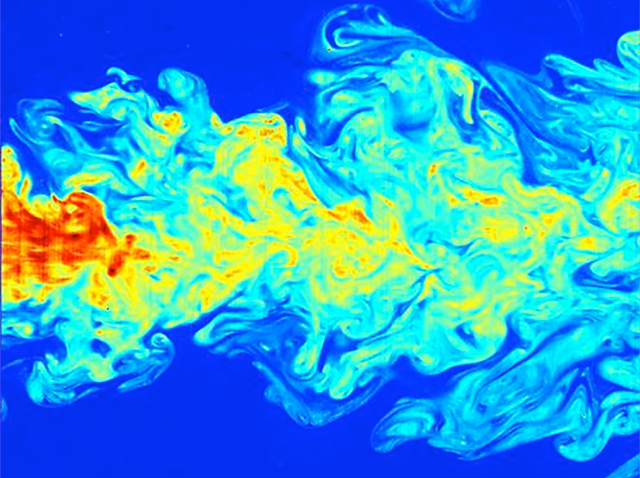
\includegraphics[width=0.55\paperwidth]{image1.png}
  	}
%  	\caption{Fluid flow}\label{fig:1}
	\end{figure}
	\end{frame}
  
  	\begin{frame}{Introduction (problem statement)}
  	Let $\boldsymbol{v}(x,y,t)=[u(x,y,t),v(x,y,t)]^T$ and $\boldsymbol{p}(x,y,t)$ be solutions to incompressible Navier-Stokes system of equations on 2D domain $\Omega$ with Dirichlet Boundary conditions on $\partial\Omega$.
	\begin{subequations}
	\label{eqs:NSE}
	\begin{align}
	\label{eqn:momentum-intro}
	\underbrace{\frac{\partial \boldsymbol{v}}{\partial t}}_{\text{transient}} 
		+ \underbrace{\boldsymbol{v} \cdot \nabla \boldsymbol{v}}_{\text{advective}} 
		&= \underbrace{-\frac{1}{\rho}\nabla p}_{\text{pressure gradient}} 
		+ \underbrace{\frac{\mu}{\rho} \nabla \cdot \nabla \boldsymbol{v}}_{\text{viscous, Laplacian}}\quad\text{(momentum) in }\Omega\\
	\label{eqn:continuity}
	\nabla \cdot \boldsymbol{v} &= 0\quad\text{(continuity) in }\Omega,\\
%	\boldsymbol{v}(\xi(s,t)) &= \int_x\boldsymbol{v}(x)\delta(x - \xi)dx = \boldsymbol{v}_B(\xi(x,t)).
	\boldsymbol{v}&=\boldsymbol{v}(x,y,t)\quad\text{on }\partial\Omega,
	\end{align}
	\end{subequations}
	where $\rho$ - density, $\mu$ - dynamic viscosity.
  \end{frame}
  
  \begin{frame}{Introduction (nondimensionalization)}
  
  After introducing the following dimensionless variables (marked with prime ${ }^{\prime}$ ):
\begin{equation*}
	x\to Lx^{\prime},  \quad 
	\boldsymbol{v}\to U_0\boldsymbol{v}^{\prime}, \quad 
	\nabla\to \frac{1}{L}\nabla^{\prime}, \quad 
%	\Delta \to \frac{1}{L^2} \Delta^{\prime},  \quad 
	p\to p^{\prime} \rho U_0^2, \quad 
	t\to \frac{L}{U_0}t^{\prime},
\end{equation*}
and Reynolds number 
\begin{equation*}
\operatorname{Re}=\frac{\rho L U_0}{\mu},
\end{equation*}
we obtain the non-dimensional momentum and continuity equations (dropped prime superscript)
	\begin{align}\label{eqs:NSE-nondim}
	\begin{split}
		\frac{\partial \boldsymbol{v}}{\partial t} + \boldsymbol{v} \cdot \nabla \boldsymbol{v} &= -\nabla p + \frac{1}{\operatorname{Re}} \nabla \cdot \nabla \boldsymbol{v},\\
		\nabla \cdot\boldsymbol{v}&=0.
	\end{split}
	\end{align}
  \end{frame}


  
  
  

  
%	\section{Discretization.\\ Transient (time), spatial (space)}
	
	\begin{frame}{Discretization (discrete operators)}
	Denote discrete spatial operators as:
\begin{enumerate}
	\item[$\hat{L}$]:  Laplacian.
	\item[$\hat{G}$]: Gradient.
	\item[$\hat{D}$]: Divergence.
	\item[$\mathbf{\hat{H}}$]: Non-linear advective terms.
\end{enumerate}
Then initial system \eqref{eqs:NSE-nondim} can be rewritten using these operators as
\begin{equation}\label{eqn:nse-matrix}
            \begin{bmatrix}
                  \mathbf{I} && 0 \\ 
                  0 && 0
            \end{bmatrix}
            \frac{\partial }{\partial t} 
            \begin{pmatrix}
                  \boldsymbol{v} \\ 
                  p
            \end{pmatrix}
            +
            \begin{pmatrix}
                  \mathbf{\hat{H}}(\boldsymbol{v})\\
                  0
            \end{pmatrix}
            =
            \begin{bmatrix}
                  \hat{L} && - \hat{G} \\ 
                  -\hat{D} && 0
            \end{bmatrix}
            \begin{bmatrix}
                  \boldsymbol{v} \\
                  p
            \end{bmatrix}
             + \text{bc}_{\boldsymbol{v},p},
        \end{equation}	
	\end{frame}
	
	
	\begin{frame}{Discretization (transient)}
	Attack \eqref{eqn:nse-matrix} with the following schemes as in Colonius (2008) (superscript denotes the time step):
\begin{enumerate}
	\item[\textbf{Viscous}] - Implicit trapezoidal - Crank Nicholson scheme (second-order in time).  
	\begin{equation}\label{eqn:viscous-crank-nicholson}
  		\hat{L}\boldsymbol{v}=\frac{1}{2}\left(\hat{L}\boldsymbol{v}^{n+1}+\hat{L}\boldsymbol{v}^n\right)
	\end{equation}

	\item[\textbf{Nonlin.}] - Explicit Adams-Bashforth (second-order in time).
	\begin{equation}\label{eqn:nonlinear-adams-bashforth}
		\mathbf{\hat{H}}(\boldsymbol{v}) = \frac{3}{2}\mathbf{\hat{H}}(\boldsymbol{v}^{n}) - \frac{1}{2}\mathbf{\hat{H}}(\boldsymbol{v})^{n-1}.
	\end{equation}

	\item[\textbf{Pressure}] - Implicit Euler (first-order in time). 
	\begin{equation}\label{eqn:pressure-implicit-euler} 
		\hat{G}p = \hat{G}p^{n+1}.
	\end{equation}
	\end{enumerate}
	\end{frame}
	
	\begin{frame}{Discretization (transient)}
	The above schemes result in the following time-discretized system:
	\begin{multline}
		\begin{bmatrix}
			\frac{1}{\Delta t}\mathbf{I}-\frac{1}{2}\hat{L} & \hat{G} \\
			\hat{D} & 0
		\end{bmatrix}
		\begin{pmatrix}
			\boldsymbol{v}^{n+1} \\ 
			p^{n+1}
		\end{pmatrix}=\\
		=
		\begin{pmatrix}
			\left[\frac{1}{\Delta t}\mathbf{I}-\frac{1}{2}\hat{L}\right] \boldsymbol{v}^n - \left[\frac{3}{2}\hat{\mathbf{H}}(\boldsymbol{v}^n) - \frac{1}{2}\hat{\mathbf{H}}(\boldsymbol{v}^{n-1})\right]\\
			0
		\end{pmatrix}
		+
		\begin{pmatrix}
			\hat{bc}_1^n\\
			\hat{bc}_2^n
		\end{pmatrix},
	\end{multline}	
	
	which in short becomes
	
	\begin{equation}\label{eqn:NSE-dsm-bl-system-nonint}
	\boxed{\begin{bmatrix}
		\hat{A} & \hat{G} \\
		\hat{D} & 0
	\end{bmatrix}
	\begin{pmatrix}
		\boldsymbol{v}^{n+1} \\ 
		p^{n+1}
	\end{pmatrix}
	=
	\begin{pmatrix}
		\hat{r}^n \\
		0
	\end{pmatrix}
	+
	\begin{pmatrix}
		\hat{bc}_1^n\\
		\hat{bc}_2^n
	\end{pmatrix}}.
	\end{equation}
	\end{frame}

	
	
	\begin{frame}{Discretization (spatial)}
		\begin{figure}[H] % here, bottom, top
		\centering{
		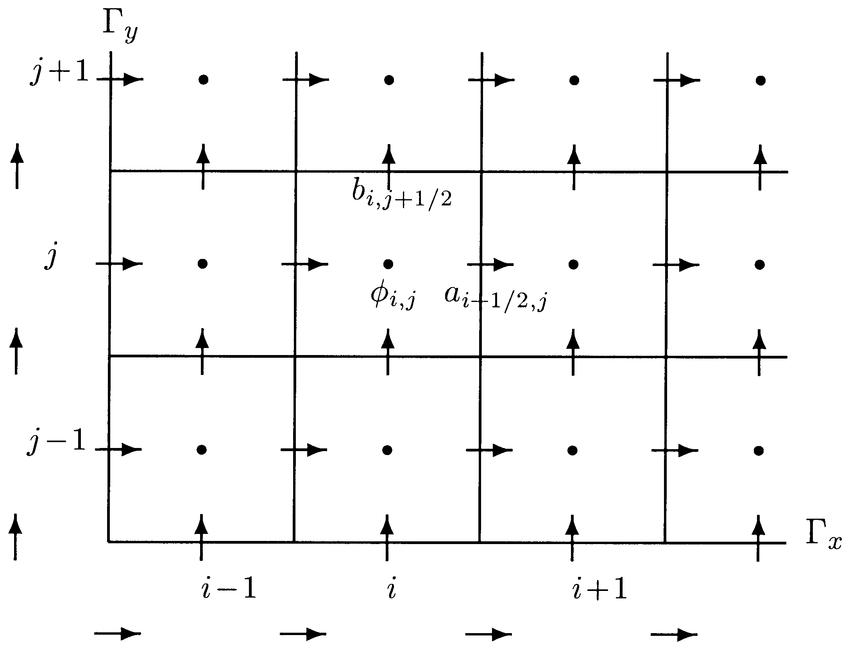
\includegraphics[width=0.75\paperwidth]{fig1}
		}
		\caption{Domain discretization as per Harlow and Welch (1965)}\label{bl-domain-discretization}
		\end{figure}
	\end{frame}
	
	\begin{frame}{Discretization (spatial Laplacian)}
	
	Rewrite Laplacian as a block matrix:
	\begin{equation*}
		\hat L=
		\begin{bmatrix}
	  \hat{L}^u_{xx}+\hat{L}^u_{yy} & 0 \\
	  0 & \hat{L}^v_{xx}+\hat{L}^v_{yy}
	\end{bmatrix}.
	\end{equation*}
	
	Use Taylor expansion to derive second derivative approximation
	\begin{multline}\label{eqn:Taylor right} 
		u_{i-\frac{1}{2}+1,j}=u_{i-\frac{1}{2},j}+\left.\frac{\partial u}{\partial x}\right|_{i-\frac{1}{2},j}\left(x_{i-\frac{1}{2}+1}-x_{i-\frac{1}{2}}\right)+\\
		+\frac{1}{2}\left.\frac{\partial^2 u}{\partial x^2}\right|_{i-\frac{1}{2},j}\left(x_{i-\frac{1}{2}+1}-x_{i-\frac{1}{2}}\right)^2+O\left(\Delta x^3\right),
	\end{multline}
	\begin{multline}\label{eqn:Taylor left} 
		u_{i-\frac{1}{2}-1,j}=u_{i-\frac{1}{2},j}+\left.\frac{\partial u}{\partial x}\right|_{i-\frac{1}{2},j}\left(x_{i-\frac{1}{2}-1}-x_{i-\frac{1}{2}}\right)+\\
		+\frac{1}{2}\left.\frac{\partial^2 u}{\partial x^2}\right|_{i-\frac{1}{2},j}\left(x_{i-\frac{1}{2}-1}-x_{i-\frac{1}{2}}\right)^2+O\left(\Delta x^3\right).
	\end{multline}
	\end{frame}
	
	\begin{frame}{Discretization (spatial Laplacian)}
	\begin{align}\label{eqn:laplacian-discretization-non-uniform-dx}
	\left.\frac{\partial^2 u}{\partial x^2}\right|_{i-\frac{1}{2},j} & \approx \frac{1}{h_c h_e}u_{i-\frac{1}{2}+1} - \frac{2}{h_w h_e}u_{i-\frac{1}{2}} + \frac{1}{h_c h_w}u_{i-\frac{1}{2}-1} + O(\Delta x),
	\end{align}	
	where $h_w=x_{i-\frac{1}{2}}-x_{i-\frac{1}{2}-1},h_c = \frac{x_{i-\frac{1}{2}+1}-x_{i-\frac{1}{2}-1}}{2}, h_e = x_{i-\frac{1}{2}+1}-x_{i-\frac{1}{2}}$.
	\end{frame}


	\begin{frame}{Discretization (spatial Laplacian at boundary)}
	
	\subsubsection{Left boundary}\label{subsubsec:laplacian-left}
	The exact value on the left boundary ($u_{\frac{1}{2},j}$) is known.
	\begin{figure}[H] % here, bottom, top
	  \centering{
	  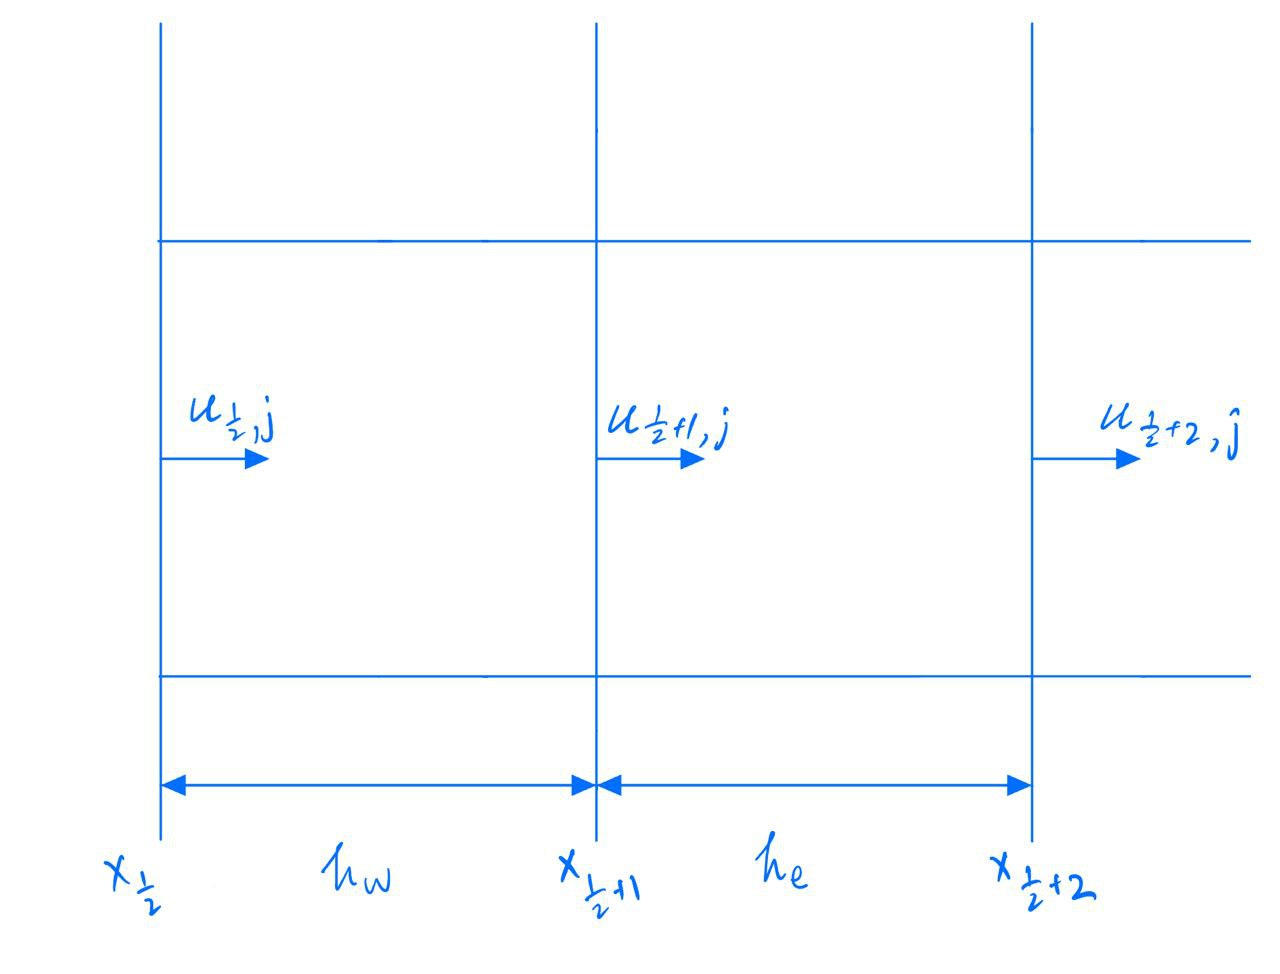
\includegraphics[width=0.55\paperwidth]{Luxx-left}
	  }
	  \caption{$\hat{L}^u_{xx}$ at the left boundary.}\label{fig:luxx-left}
	\end{figure}
	\end{frame}
	
	\begin{frame}{Discretization (spatial Laplacian at boundary)}
	\begin{figure}[H]
	\centering{
	  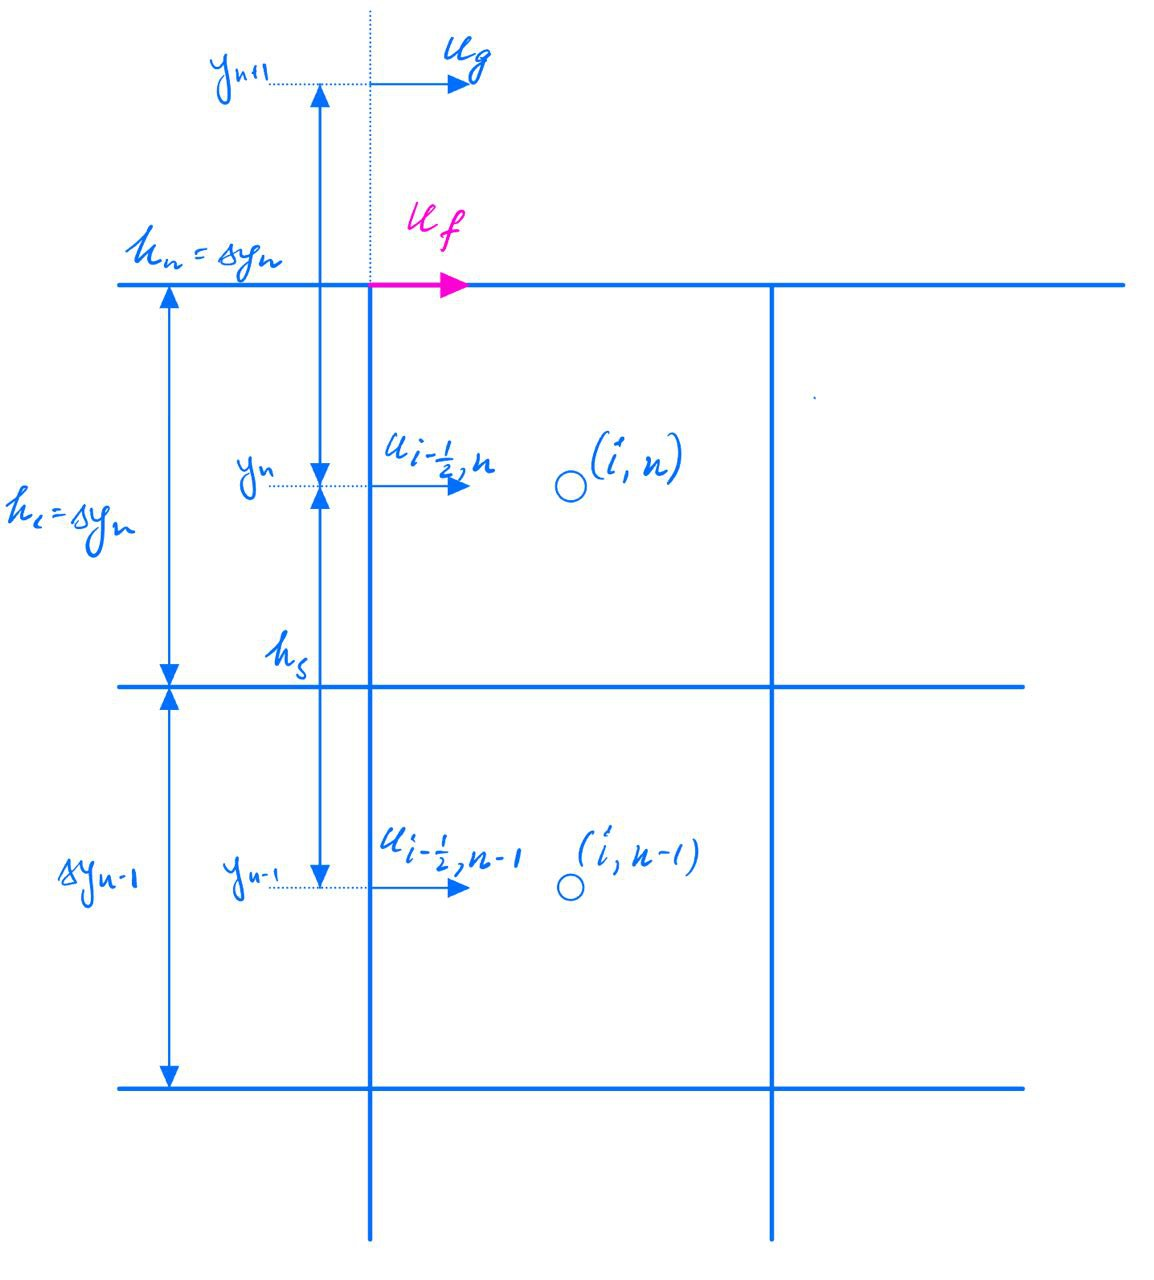
\includegraphics[width=0.35\paperwidth]{Luxx-top.jpg}
	  }
	  \caption{$\hat{L}^u_{yy}$ at top boundary.}\label{fig:luxx-top}
	\end{figure}	
	$u_{f} = \frac{u_g+u_{i-\frac{1}{2},N}}{2}\implies u_g=2u_{f}-u_{i-\frac{1}{2},N}\implies$
	$\left.\frac{\partial^2 u}{\partial y^2}\right|_{i-\frac{1}{2},N}=\frac{2 u_f}{h_c{ }^2}+u_{i-\frac{1}{2},N}\left(\frac{-\left(2 h_c+h_s\right)}{h_c^2 h_s}\right)+u_{i-\frac{1}{2},N-1} \frac{1}{h_s h_c}.$
	\end{frame}
	
	\begin{frame}{Discretization (spatial advection)}
	Advection in conservative form allows to compute derivatives with simple second order central difference formula $\left.\frac{\partial u}{\partial x}\right|_{i}=\frac{u_{i+1}-u_{i-1}}{x_{i+1}-x_{i-1}}$:
		\begin{align}\label{eqn:advection-conservative}
		u\frac{\partial u}{\partial x}+v \frac{\partial u}{\partial y}
		&=u\frac{\partial u}{\partial x}+0+v \frac{\partial u}{\partial y}\nonumber\\
		&= u\frac{\partial u}{\partial x}+ u\left(\frac{\partial u}{\partial x} +\frac{\partial v}{\partial y}\right ) +v \frac{\partial u}{\partial y}\nonumber\\
		&=\left(u\frac{\partial u}{\partial x}+ u\frac{\partial u}{\partial x}\right ) +\left(u\frac{\partial v}{\partial y} +v \frac{\partial u}{\partial y}\right )\nonumber\\
		&=\frac{\partial uu}{\partial x}+ \frac{\partial uv}{\partial y}.
	\end{align}
	
	\end{frame}



	\begin{frame}{Discretization (spatial advection)}
	\subsubsection{Inner part}\label{subsubsec:advection-inner}
	\begin{figure}[H] % here, bottom, top
	  \centering{
	  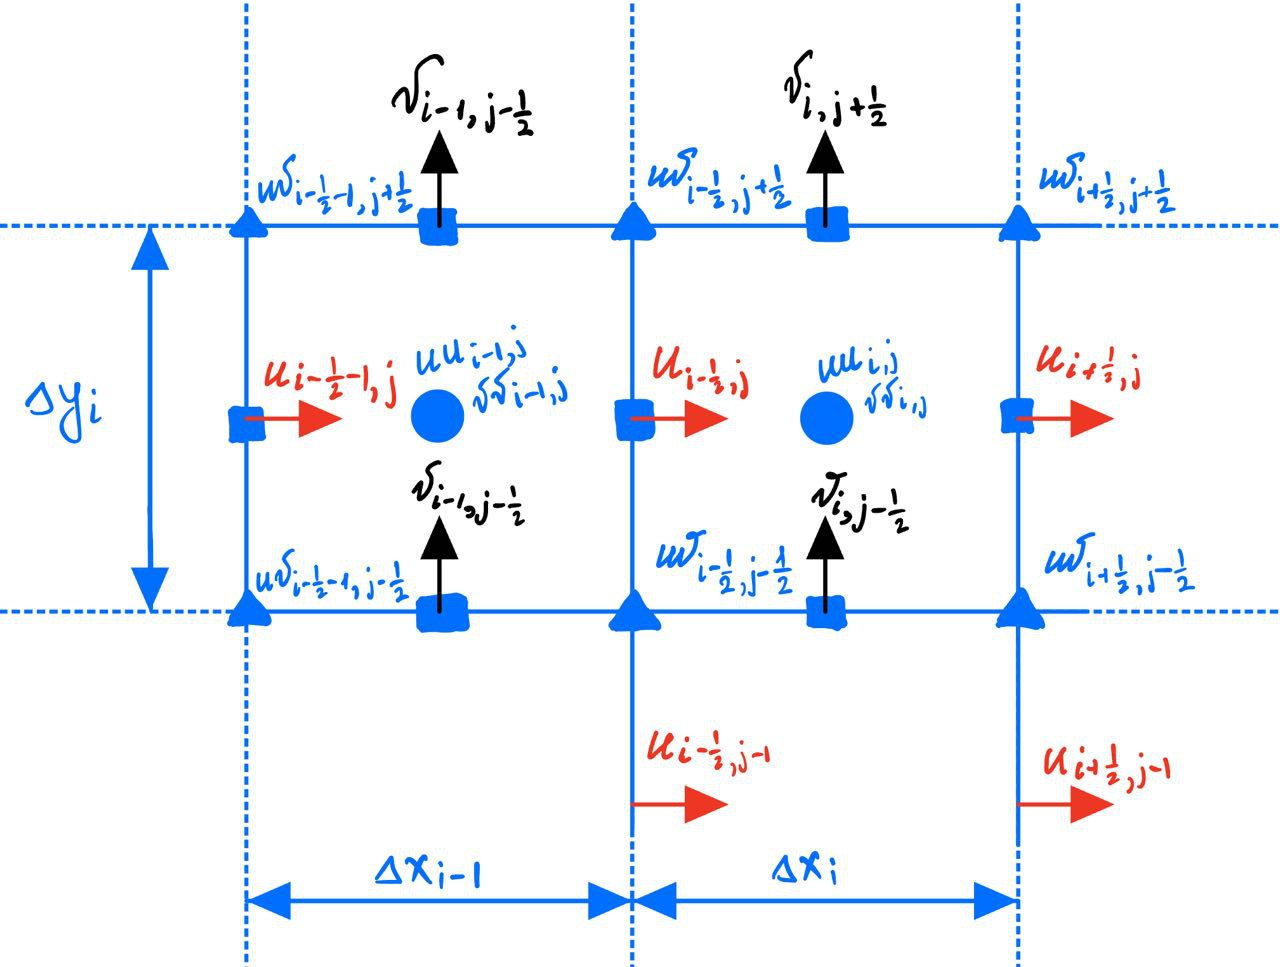
\includegraphics[width=0.65\paperwidth]{ADV}
	  }
	  \caption{Advection discretization.}\label{fig:ADV}
	\end{figure}	
	\end{frame}

	
	\begin{frame}{Discretization (divergence)}
	\begin{equation*}
	\begin{gathered}
	\hat{D}\boldsymbol{v}=\hat{bc}_2^n,\\
	\left[ 
	\begin{array}{ll}
	\hat{D}_x & \hat{D}_y 	
	\end{array}
	\right]\left[\begin{array}{l}
	u\\
	v
	\end{array}
	\right]=\hat{bc}_2^n
	, \\
	\frac{1}{\Delta x} D_x u+\frac{1}{\Delta y} D_y v=\hat{bc}_2^n, \\
	\frac{1}{\Delta _{xy}}\left[\begin{array}{ll}
	D_x & D_y
	\end{array}\right]\left[\begin{array}{l}
	u \Delta y \\
	v \Delta x
	\end{array}\right]=\frac{1}{\Delta _{xy}} D q=\hat{bc}_2^n,
	\end{gathered}
	\end{equation*}	
	where 
	\begin{equation}\label{eqn:delta-xy}
		q=\left[\begin{array}{l}
	u \Delta y \\
	v \Delta x
	\end{array}\right], \quad \Delta _{xy}=
		\begin{bmatrix}{}
			\frac{1}{\Delta x_1\Delta y_1}		&0	&\dots	&0\\
			0		&\frac{1}{\Delta x_2\Delta y_1}	&\dots	&0\\
			\vdots		&\vdots	&\ddots	&\vdots\\
			0		&0	&\dots	&\frac{1}{\Delta x_M\Delta y_N}
		\end{bmatrix}.
	\end{equation}
	
	\end{frame}
	
	\begin{frame}{Discretization (divergence)}
	\begin{figure}[H] % here, bottom, top
	  \centering{
	  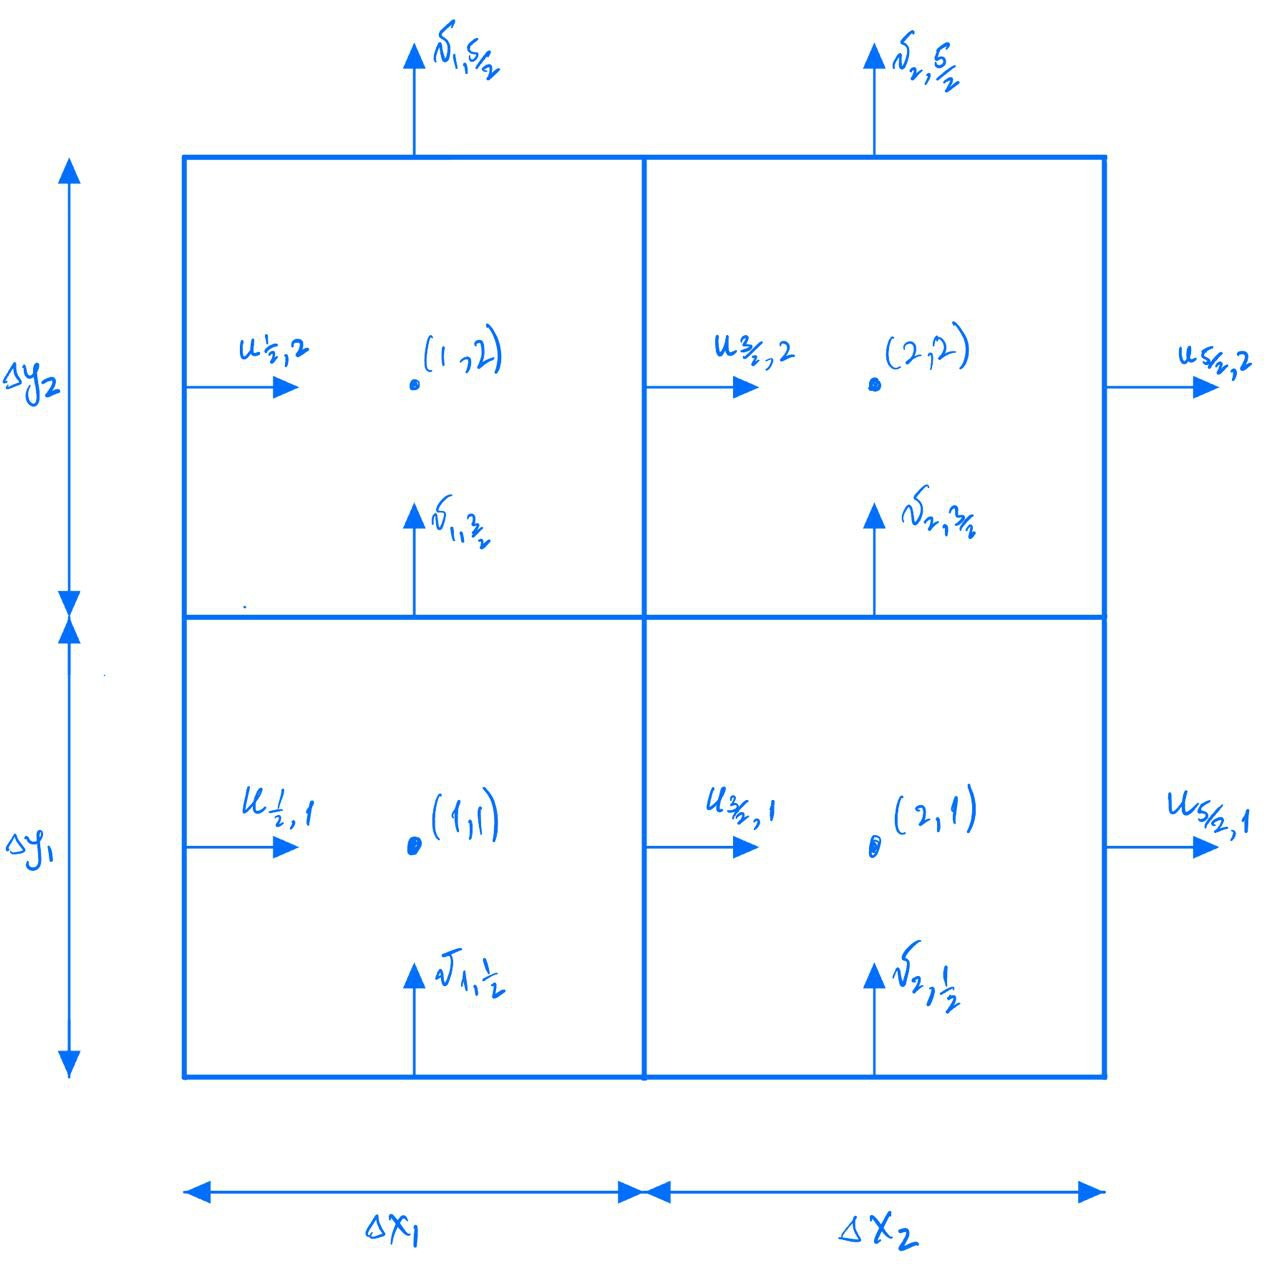
\includegraphics[width=0.55\paperwidth]{D-example-2x2}
	  }
	  \caption{$2\times 2$ grid example for divergence operator.}\label{fig:D-example-2x2}
	\end{figure}	
	\end{frame}
	
	\begin{frame}{Discretization (divergence)}
	\begin{equation}\label{eqn:divergence-matrix}
	\Delta_{xy}\left[\begin{array}{rrrrrr}
	1  & 0  & 1 & 0 \\
	-1  & 0  & 0 & 1 \\
	0  & 1  & -1 & 0 \\
	0  & -1  & 0 & -1
	\end{array}\right]\left[\begin{array}{l}
	u_{\frac{3}{2},1} \Delta y_1 \\
	u_{\frac{3}{2},2} \Delta y_2 \\
	v_{1,\frac{3}{2}} \Delta x_1 \\
	v_{2,\frac{3}{2}} \Delta x_2
	\end{array}\right]=
	\begin{bmatrix}{}
	\frac{u_{\frac{1}{2},1}}{\Delta x_1}+\frac{v_{1,\frac{1}{2}}}{\Delta y_1} \\
	\frac{u_{\frac{5}{2},1}}{\Delta x_2}+\frac{v_{2,\frac{1}{2}}}{\Delta y_1} \\
	\frac{u_{\frac{1}{2},2}}{\Delta x_1}-\frac{v_{1,\frac{5}{2}}}{\Delta y_2} \\
	\frac{u_{\frac{5}{2},2}}{\Delta x_2}-\frac{v_{2,\frac{5}{2}}}{\Delta y_2}
	\end{bmatrix}.
	\end{equation}
	\end{frame}
	
	\begin{frame}{Discretization (pressure gradient)}
		\begin{figure}[H] % here, bottom, top
		  \centering{
		  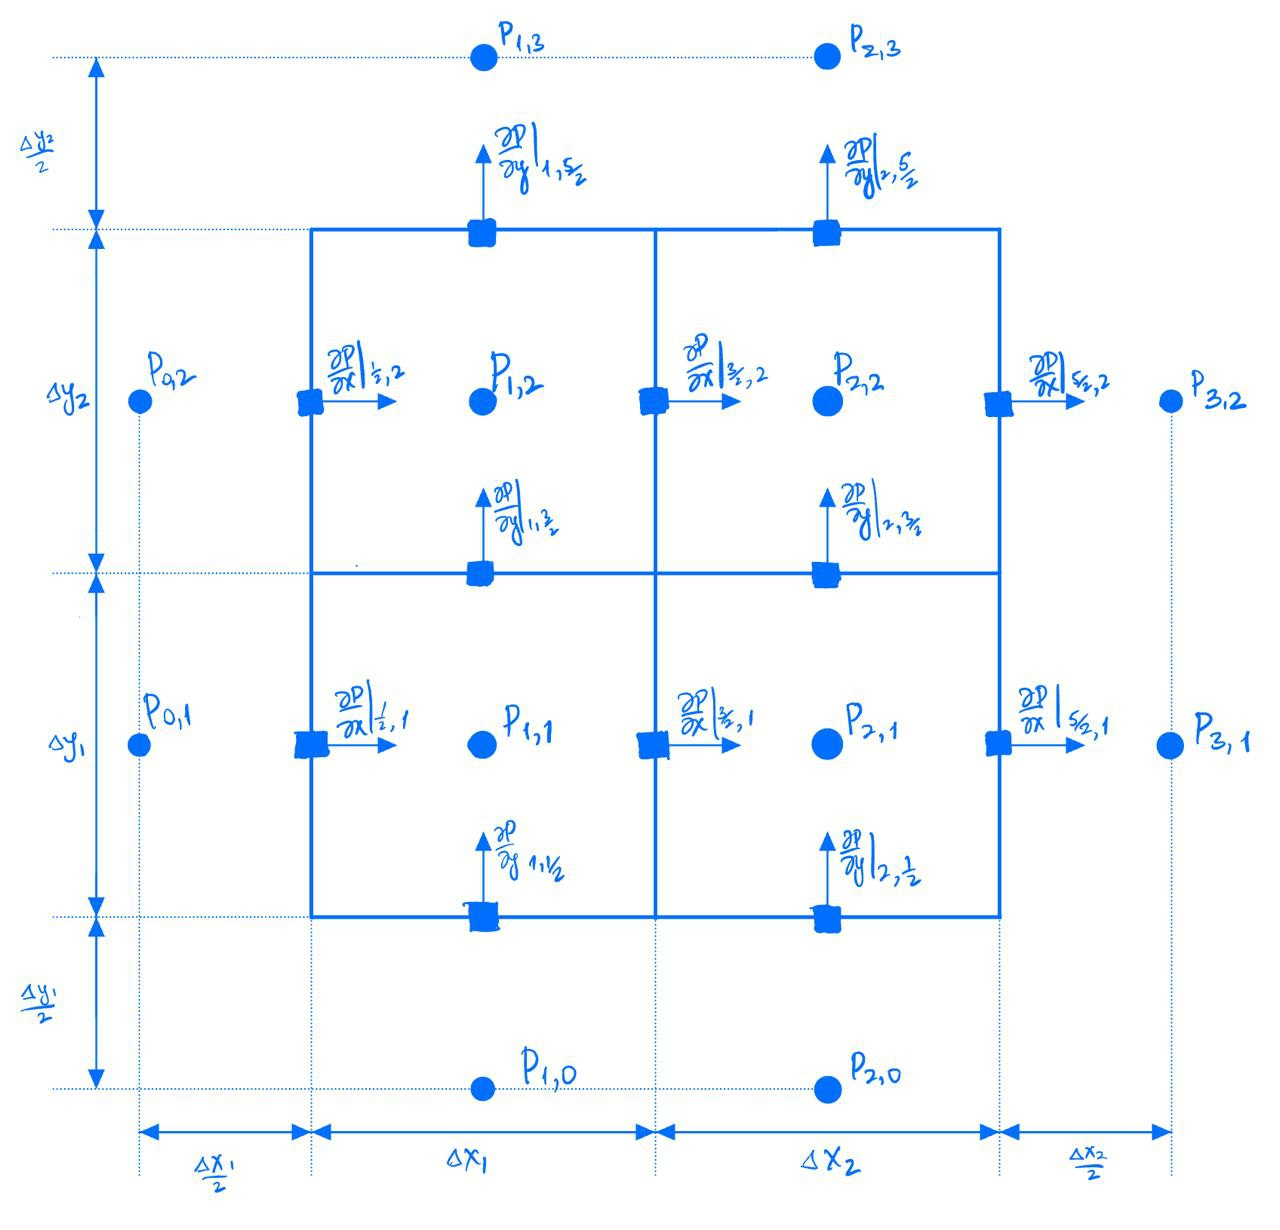
\includegraphics[width=0.55\paperwidth]{G-example-2x2}
		  }
		  \caption{$2\times 2$ grid example for gradient operator.}\label{fig:G-example-2x2}
		\end{figure}
	\end{frame}
	
	
	\begin{frame}{Discretization (pressure gradient)}
	Notice, that matrix of coefficients below is very similar to Divergence matrix, i.e. $G=-D^T$.
	\begin{equation}\label{eqn:gradient-matrix}
	diag\left[\begin{array}{cccccc}
	\frac{2}{\Delta x_1+\Delta x_2} \\
	\frac{2}{\Delta x_1+\Delta x_2} \\
	\frac{2}{\Delta y_1+\Delta y_2} \\
	\frac{2}{\Delta y_1+\Delta y_2}
	\end{array}\right]
	\left(\left[\begin{array}{rrrr}
	-1 & 1 & 0 & 0 \\
	0 & 0 & -1 & 1 \\
	-1 & 0 & 1 & 0 \\
	0 & -1 & 0 & 1
	\end{array}\right]
	\begin{bmatrix}{}
	  p_{1,1} \\
	  p_{2,1} \\
	  p_{1,2} \\
	  p_{2,2} 
	\end{bmatrix}
	+\left[\begin{array}{c}
	0 \\
	p_{3,1} \\
	0 \\
	 p_{3,2} \\
	0 \\
	0
	\end{array}\right]\right).
	\end{equation}
	\end{frame}
	
	

%	\section{Normalization.\\Making system symmetric.}
	
	\begin{frame}{Normalization. Symmetrization.}
	\begin{align*}
	R &\equiv\left[\begin{array}{cc}
	\Delta y_j & 0 \\
	0 & \Delta x_i
	\end{array}\right], \\
	\quad \hat{M} & \equiv\left[\begin{array}{cc}
	\frac{1}{2}\left(\Delta x_i+\Delta x_{i-1}\right) & 0 \\
	0 & \frac{1}{2}\left(\Delta y_j+\Delta y_{j-1}\right)
	\end{array}\right].
	\end{align*}
	
	Let $q=R\boldsymbol{v}$, then $\boldsymbol{v}=R^{-1}q$. 
	
	Left multiplication by $\hat{M}$ of momentum equation changes $\hat{M}^{-1}G$ to $G$.
	
	Left multiplication by $\hat{M}$ rescales $\hat{L}$ in one direction, right multiplication by $R^{-1}$ in another. We obtain $\hat{M}\hat{L}R^{-1}$ symmetric, $\hat{M}IR^{-1}$ diagonal, hence, $\hat{M}\hat{A}R^{-1}$ symmetric.
	\end{frame}
	
	\begin{frame}{Normalization. Symmetrization.}
	Resultant system finally becomes symmetric
		\begin{equation}\label{eqn:NSE-dsm-bl-system-nonint}
		\boxed{\begin{bmatrix}
			{A} & {G} \\
			{D} & 0
		\end{bmatrix}
		\begin{pmatrix}
			q^{n+1} \\ 
			p^{n+1}
		\end{pmatrix}
		=
		\begin{pmatrix}
			{r}^n \\
			0
		\end{pmatrix}
		+
		\begin{pmatrix}
			{bc}_1^n\\
			0
		\end{pmatrix}.}
		\end{equation}
		We will consider $\hat{bc}_2^n=0$ for Lid Driven Cavity problem. 
	\end{frame}

	


	
	
%	\section{Motivation.}
	\begin{frame}{Motivation. Is it possible to remove the need to solve for pressure in our the system?}
	Stream function $\psi(x,y,t):\boldsymbol{v}=\nabla \times \psi$ of an incompressible two-dimensional flow:
	\begin{equation}
	\label{eqn:streamfunction}
		u = \frac{\partial \psi}{\partial y},\quad v=-\frac{\partial \psi}{\partial x}.
	\end{equation}
	Vorticity $\omega = \nabla \times \boldsymbol{v}$, in two-dimensional case (x-y-plane) the only non-zero component of $\omega$ is $z$, which leads to
	\begin{equation}
	\label{eqn:vorticity}
		\omega=- \frac{\partial u}{\partial y}+\frac{\partial v}{\partial x}.
	\end{equation}
	\end{frame}
  
  \begin{frame}{Motivation. Including Poisson equation directly into our system.}
  \eqref{eqn:streamfunction} into \eqref{eqn:vorticity} leads to
	\begin{equation}
			\label{eqn:vorticity-stream}
			-\nabla ^2 \psi = \omega.
		\end{equation}
  Apply $(\nabla \times)$ to momentum. Since curl of gradient is zero, i.e.:
	\begin{equation}
	-\frac{\partial}{\partial y}\left(\frac{\partial p}{\partial x}\right)  
	+\frac{\partial}{\partial x}\left(\frac{\partial p}{\partial y}\right)=0
	\end{equation}
	we get
  \begin{equation}
			\label{eqn:transport-vorticity}
				\frac{\partial\omega}{\partial t} -\epsilon \left(\frac{\partial ^2 \omega}{\partial x^2} 
				+ \frac{\partial^2 \omega}{\partial y^2} \right)
				=-\left( u \frac{\partial\omega}{\partial x} 
				+ v\frac{\partial\omega}{\partial y}\right).
			\end{equation}
	Vorticity Streamfunciton Poisson \eqref{eqn:vorticity-stream} into Vorticity Transport \eqref{eqn:transport-vorticity}:
	\begin{equation}
	\label{eqn:biharmonic-streamfunction}
		\boxed{
		-\frac{\partial\nabla ^2 \psi}{\partial t} 
		+\epsilon\nabla ^4 \psi=\left( u \frac{\partial}{\partial x} 
				+ v\frac{\partial}{\partial y}\right)\nabla^2\psi.
		}
	\end{equation}
	\end{frame}
	
	
	
%	\section{Nullspace approach. \\}
	
	\begin{frame}{Nullspace approach (the main idea). Finding the analogue of $(\nabla \times)$ to eliminate pressure from the system.}
	Recall, that we previously found out that $G=-D^T$ by construction. Matrix $D$ is wider than tall for systems greater than $2\times 2$. (Number of cells is always less than the number of unknown velocity components.)
	
	Let matrix $C$ be nullspace of $D$, i.e. $DC\equiv0$. 
	Then $0\equiv-(DC)^T=-C^TD^T=C^TG$. Hence, $C^T$ is equivalent to $\nabla\times$. 
	\end{frame}
	
	\begin{frame}{Nullspace approach (computing matrix C)}
	\begin{equation*}
		\vcenter{\hbox{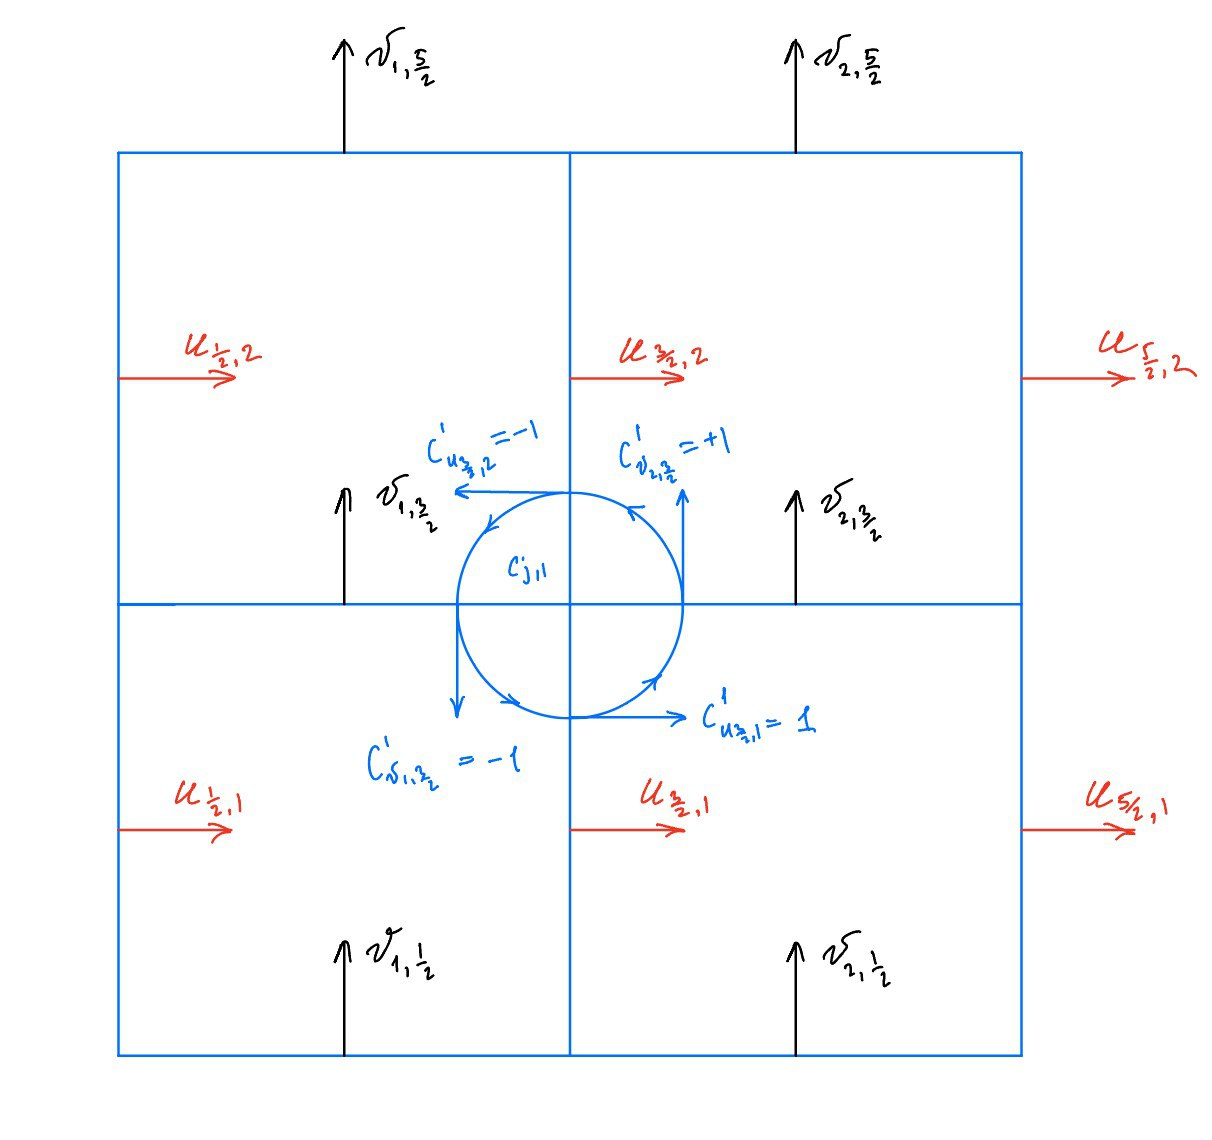
\includegraphics[width=0.60\paperwidth]{C-example-2x2}}}\quad
		C = 
  \left[\begin{array}{c}
  1		\\
  -1	\\
  -1	\\
  1		\\
\end{array}\right]
	\end{equation*}
	\end{frame}
	

	
%	\section{Algorithm}
	
	\begin{frame}{Algorithm}
		The motivation is to multiply the system 
		\begin{equation}\label{eqn:NSE-dsm-bl-system-nonint}
		{\begin{bmatrix}
			{A} & {G} \\
			{D} & 0
		\end{bmatrix}
		\begin{pmatrix}
			q^{n+1} \\ 
			p^{n+1}
		\end{pmatrix}
		=
		\begin{pmatrix}
			{r}^n \\
			0
		\end{pmatrix}
		+
		\begin{pmatrix}
			{bc}_1^n\\
			0
		\end{pmatrix}}
		\end{equation}
	by $C^T$ in order to eliminate the pressure. If we are to keep system symmetric, then need to make substitution $q=C\psi$, which results in  
		\begin{equation}\label{eqn:NSE-dsm-bl-system-nonint}
		{\begin{bmatrix}
			{C^TA} & {C^TG} \\
			{D} & 0
		\end{bmatrix}
		\begin{pmatrix}
			C\psi^{n+1} \\ 
			p^{n+1}
		\end{pmatrix}
		=
		\begin{pmatrix}
			C^T{r}^n \\
			0
		\end{pmatrix}
		+
		\begin{pmatrix}
			C^T{bc}_1^n\\
			0
		\end{pmatrix}}.
		\end{equation}
		Automatically satisfies continuity $DC\psi\equiv 0$.
		
	\end{frame}
	
	\begin{frame}{Algorithm}
	\begin{enumerate}
		\item Construct $\operatorname{curl}$ matrix $C$, such that $DC=0$ and $q_h=C\psi$.
		\item Eliminate the pressure terms in the momentum equation.
		\begin{align}
			Aq^{n+1}&=D^Tp^{n+1}+bc_1, &\text{ premultiply by $C^T$,} \notag\\
			C^TAq^{n+1}&=C^Tbc_1, &\text{ use $q^{n+1}=C\psi^{n+1}$,}\notag\\
			C^TAC\psi^{n+1}&=C^Tbc_1\label{eqn:resulting-system}.&\text{solve symmetric system for $\psi^{n+1}$.}
		\end{align}
		\item Obtain $q^{n+1}=C\psi^{n+1}$. Update $bc_1$ if needed, recompute RHS. 
		\item Repeat steps (2)-(3) for $n+2$
	\end{enumerate}
	\end{frame}
	
%	\section{Results for Lid Driven Cavity Flow}
	
	\begin{frame}{Results for Lid Driven Cavity Flow}
	\begin{figure}
	\centering
	  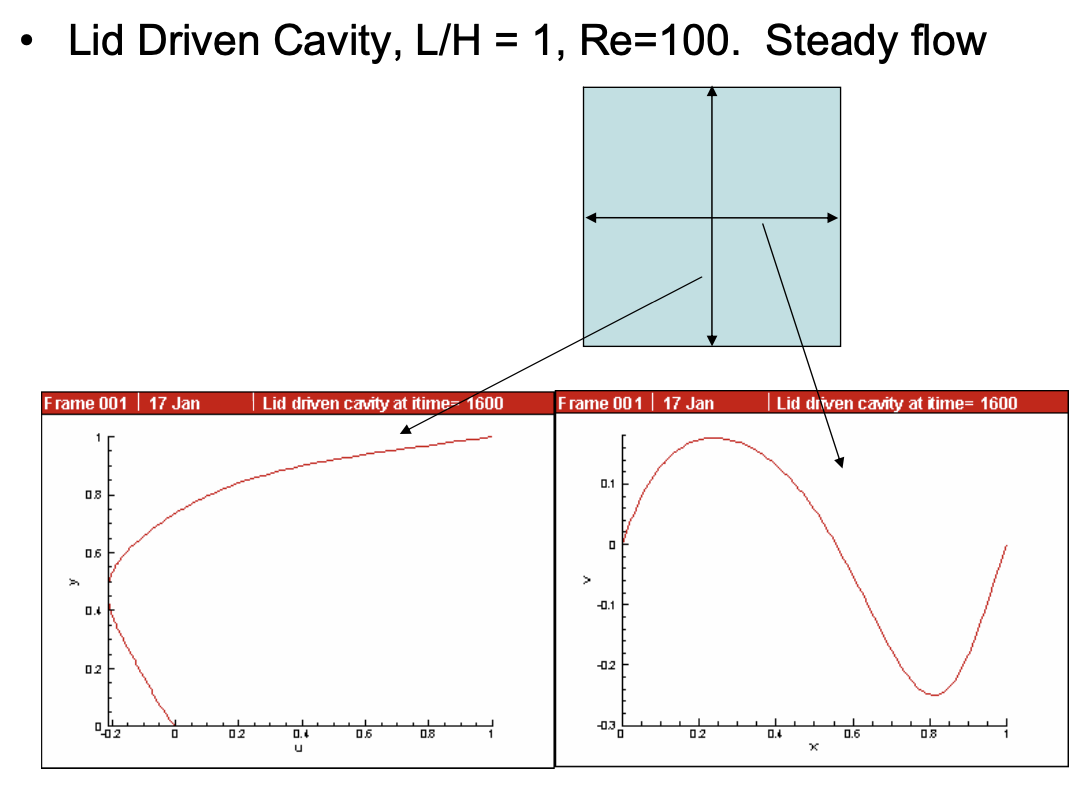
\includegraphics[height=0.395\textwidth]{fig2}
	  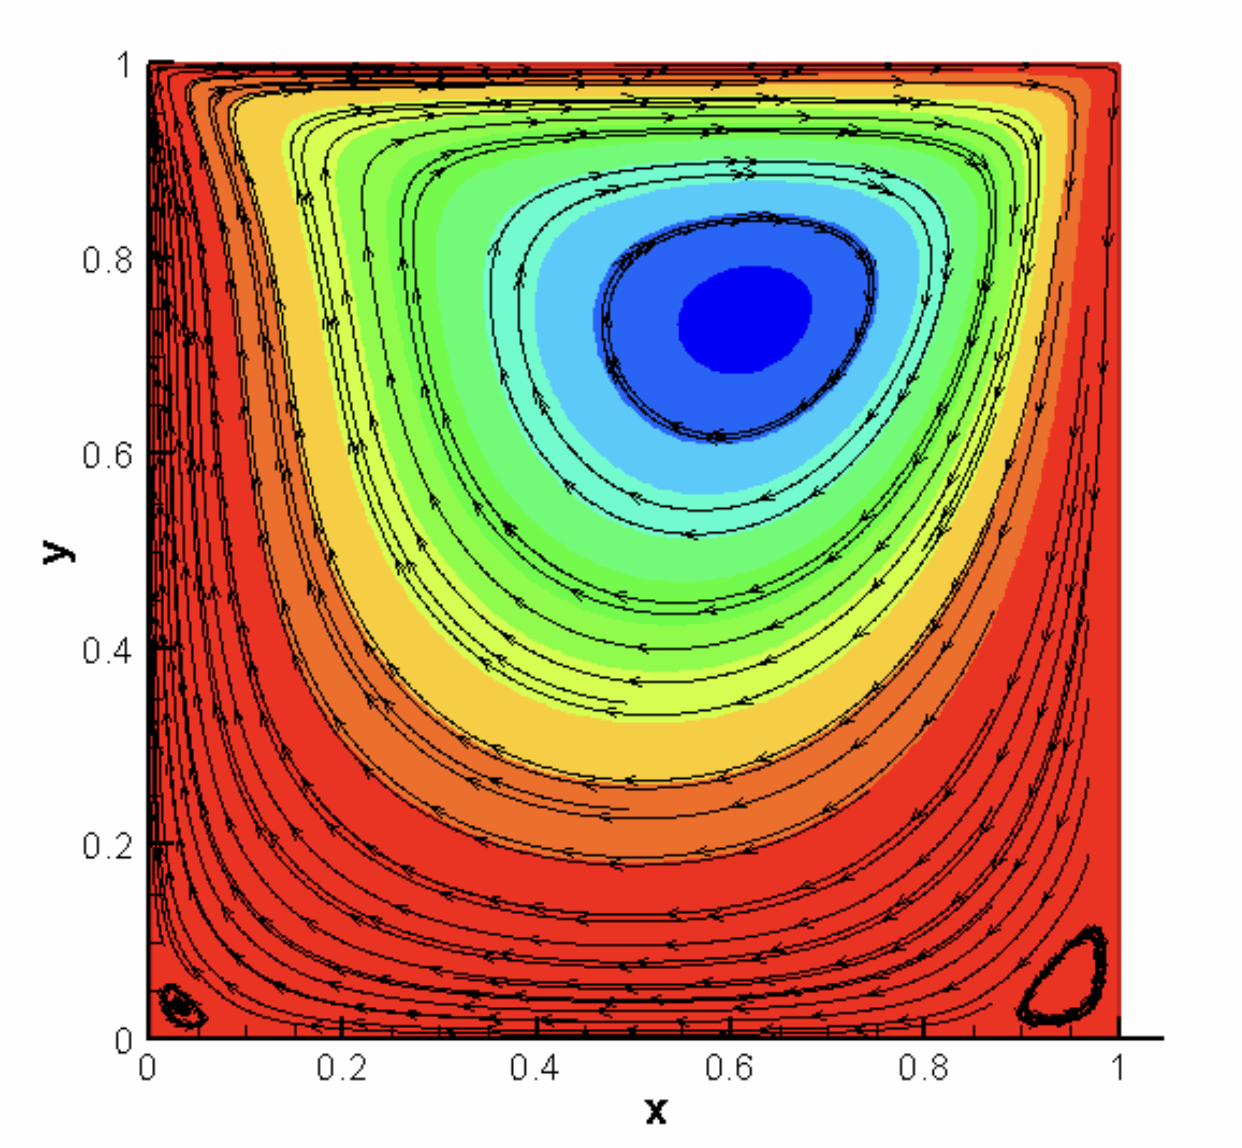
\includegraphics[height=0.395\textwidth]{fig3}\caption{Velocities perpendicular to the the middle axises and streamfunction contour at Re=1600.}
	\end{figure}
	\end{frame}
	
	\begin{frame}{Future work}
	
	We considered $\hat{bc}_2^n=0$ for Lid Driven Cavity problem in continuity equation.
	
	Other types of BCs. Multi-domain approach.
	\begin{figure}[H] % here - h, bottom - b, top - t
  \centering{
  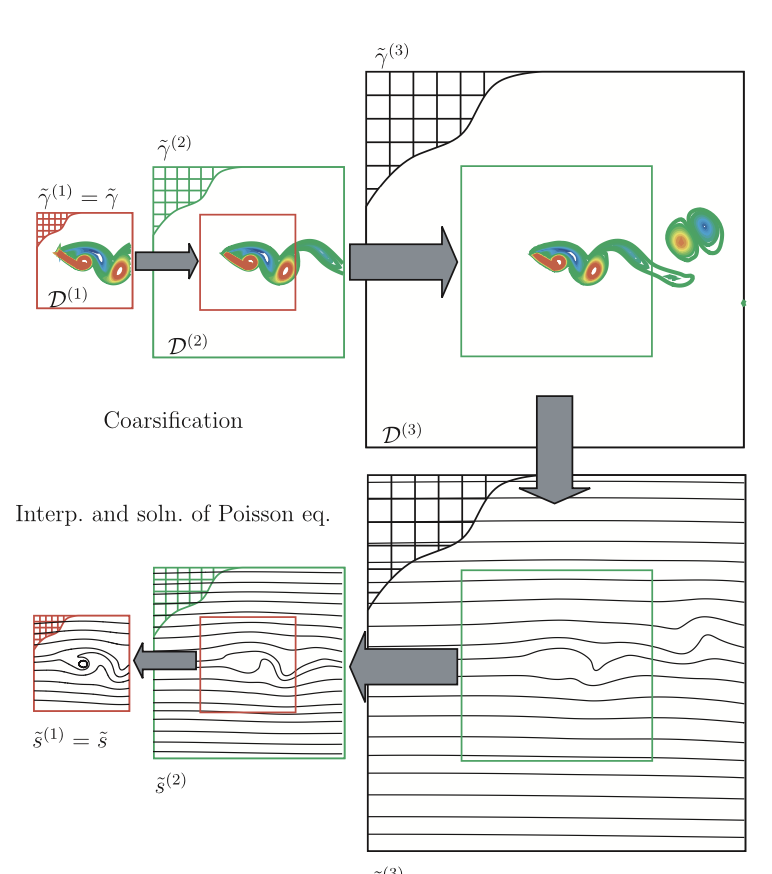
\includegraphics[width=0.40\paperwidth]{fig4}
  }
  \caption{}\label{fig:}
\end{figure}

		
	\end{frame}
	
	
	
	
	
	
\end{document}